\chapter{Utilizzo di MegAlexa}
\label{utilizzo}

\section{Creazione Workflow}
Al primo avvio dell'applicazione apparirà una schermata vuota, priva di \textit{workflow$_{G}$}.
\begin{enumerate}
\item Cliccare sul tasto "+" per aggiungere un nuovo workflow.
	\begin{figure}[h]
		\centering
		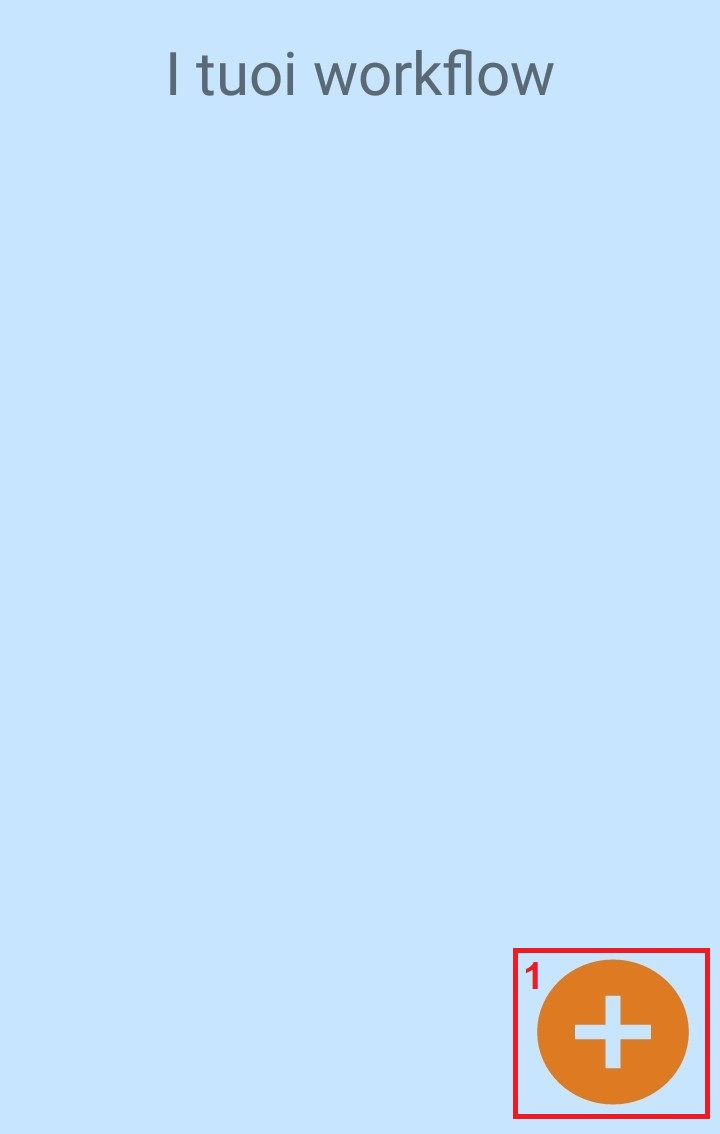
\includegraphics[scale=0.2]{images/HomeWorkflowEmpty.jpg}
		\caption{Elenco workflow vuoto}
	\end{figure}
	\newpage
\item Inserire il nome del nuovo workflow nell'apposito campo di testo ed infine premere l'icona in alto a destra per salvare.\\
\textbf{NOTA BENE:} all'utente non è permesso creare due o più workflow con lo stesso nome.

\begin{figure}[!ht]
	\centering
	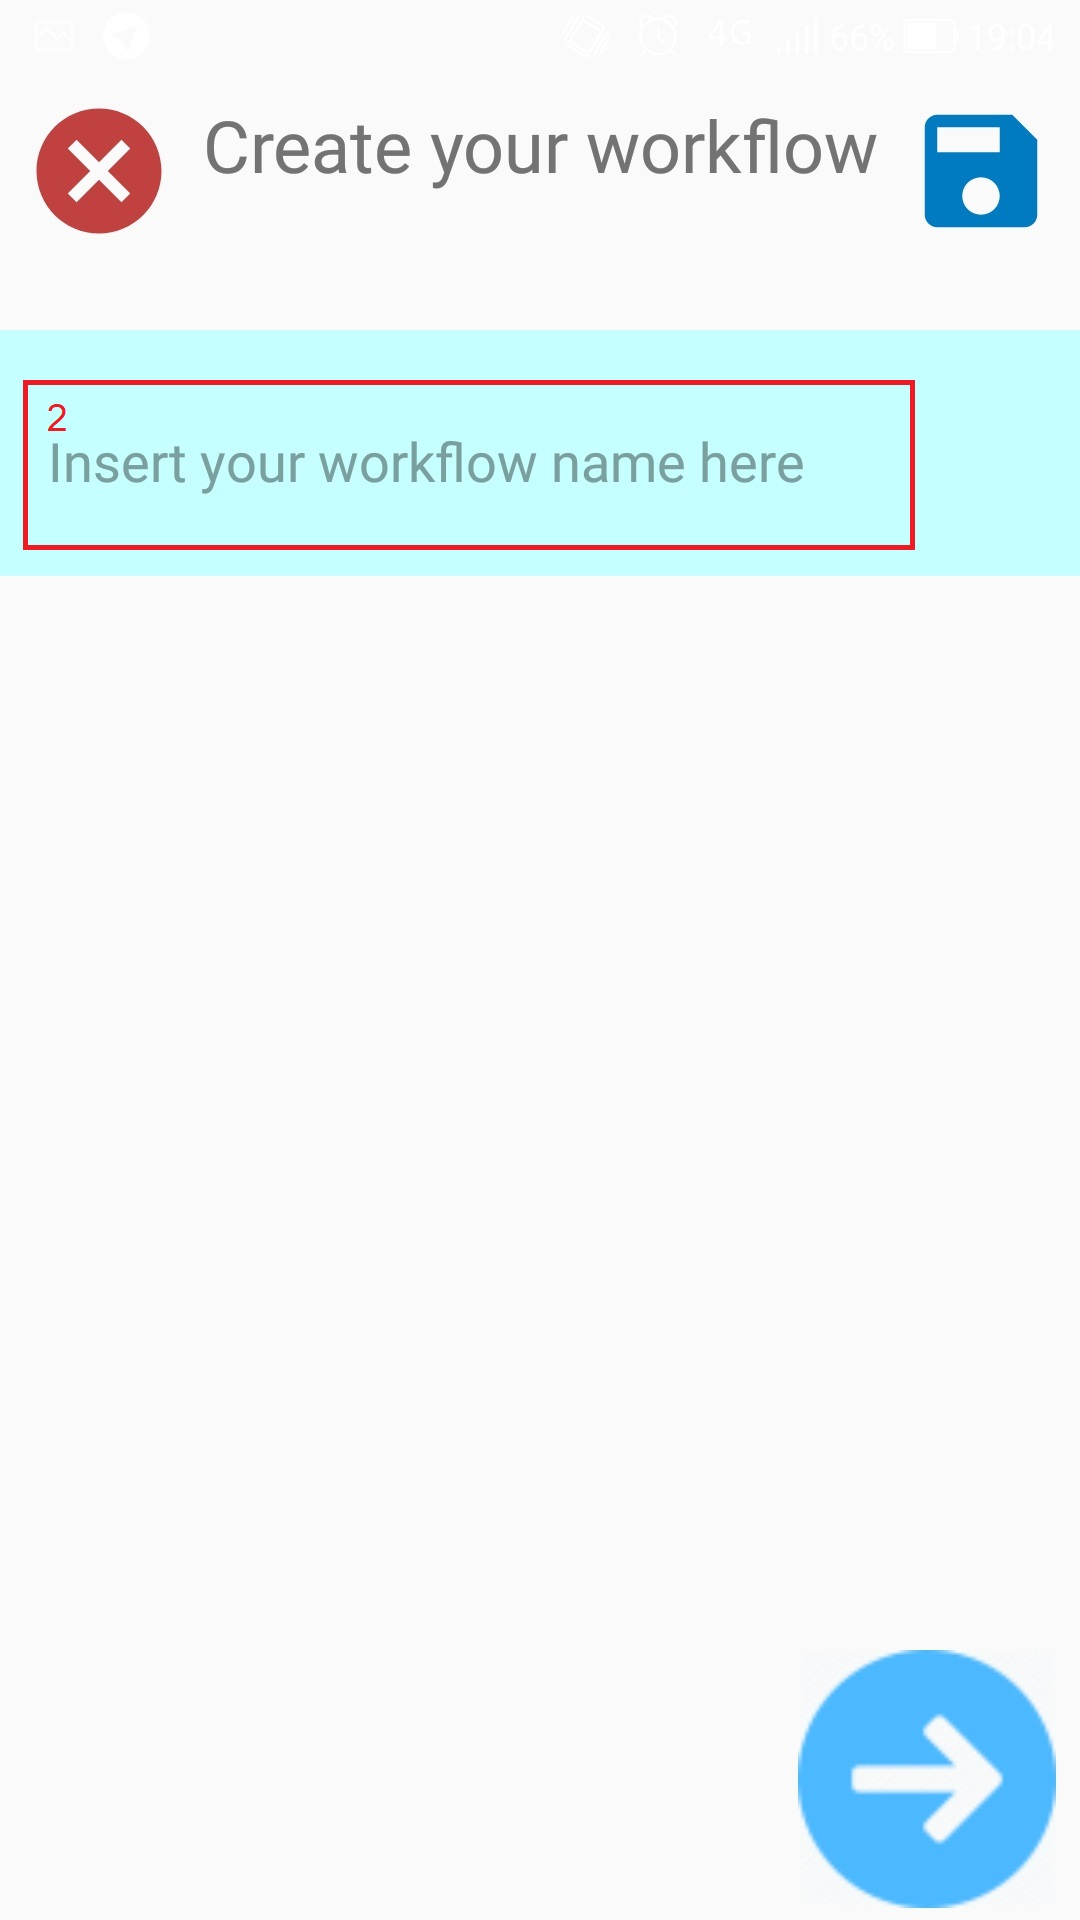
\includegraphics[scale=0.2]{images/AddWorkflow.jpg}
	\caption{Schermata aggiunta workflow}
\end{figure}
\newpage
\item Nell'elenco dei workflow, a questo punto, si potrà vedere il nuovo workflow appena creato.

\begin{figure}[!ht]
	\centering
	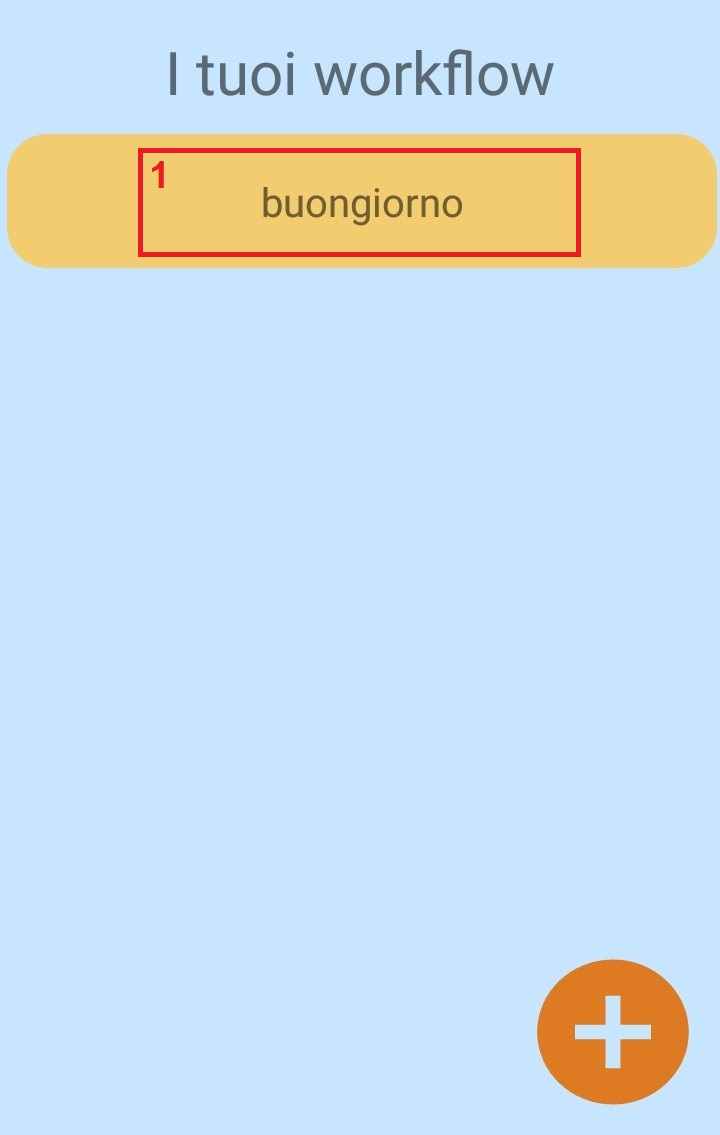
\includegraphics[scale=0.2]{images/HomeWorkflow.jpg}
	\caption{Elenco workflow con il nuovo workflow creato}
\end{figure}
\end{enumerate}
\newpage
\subsection{Aggiunta blocchi}
Una volta creato il workflow apparirà vuoto, senza blocchi.
I seguenti punti spiegheranno dettagliatamente come aggiungere i vari tipi di blocchi al \textit{workflow$_{G}$}.

\textbf{NOTA BENE:} all'interno di un workflow non è consentito inserire due o più blocchi dello stesso tipo.
Cliccando sul workflow creato nel punto precedente verrà mostrata la lista di tutti i blocchi disponibili.

\begin{figure}[!ht]
	\centering
	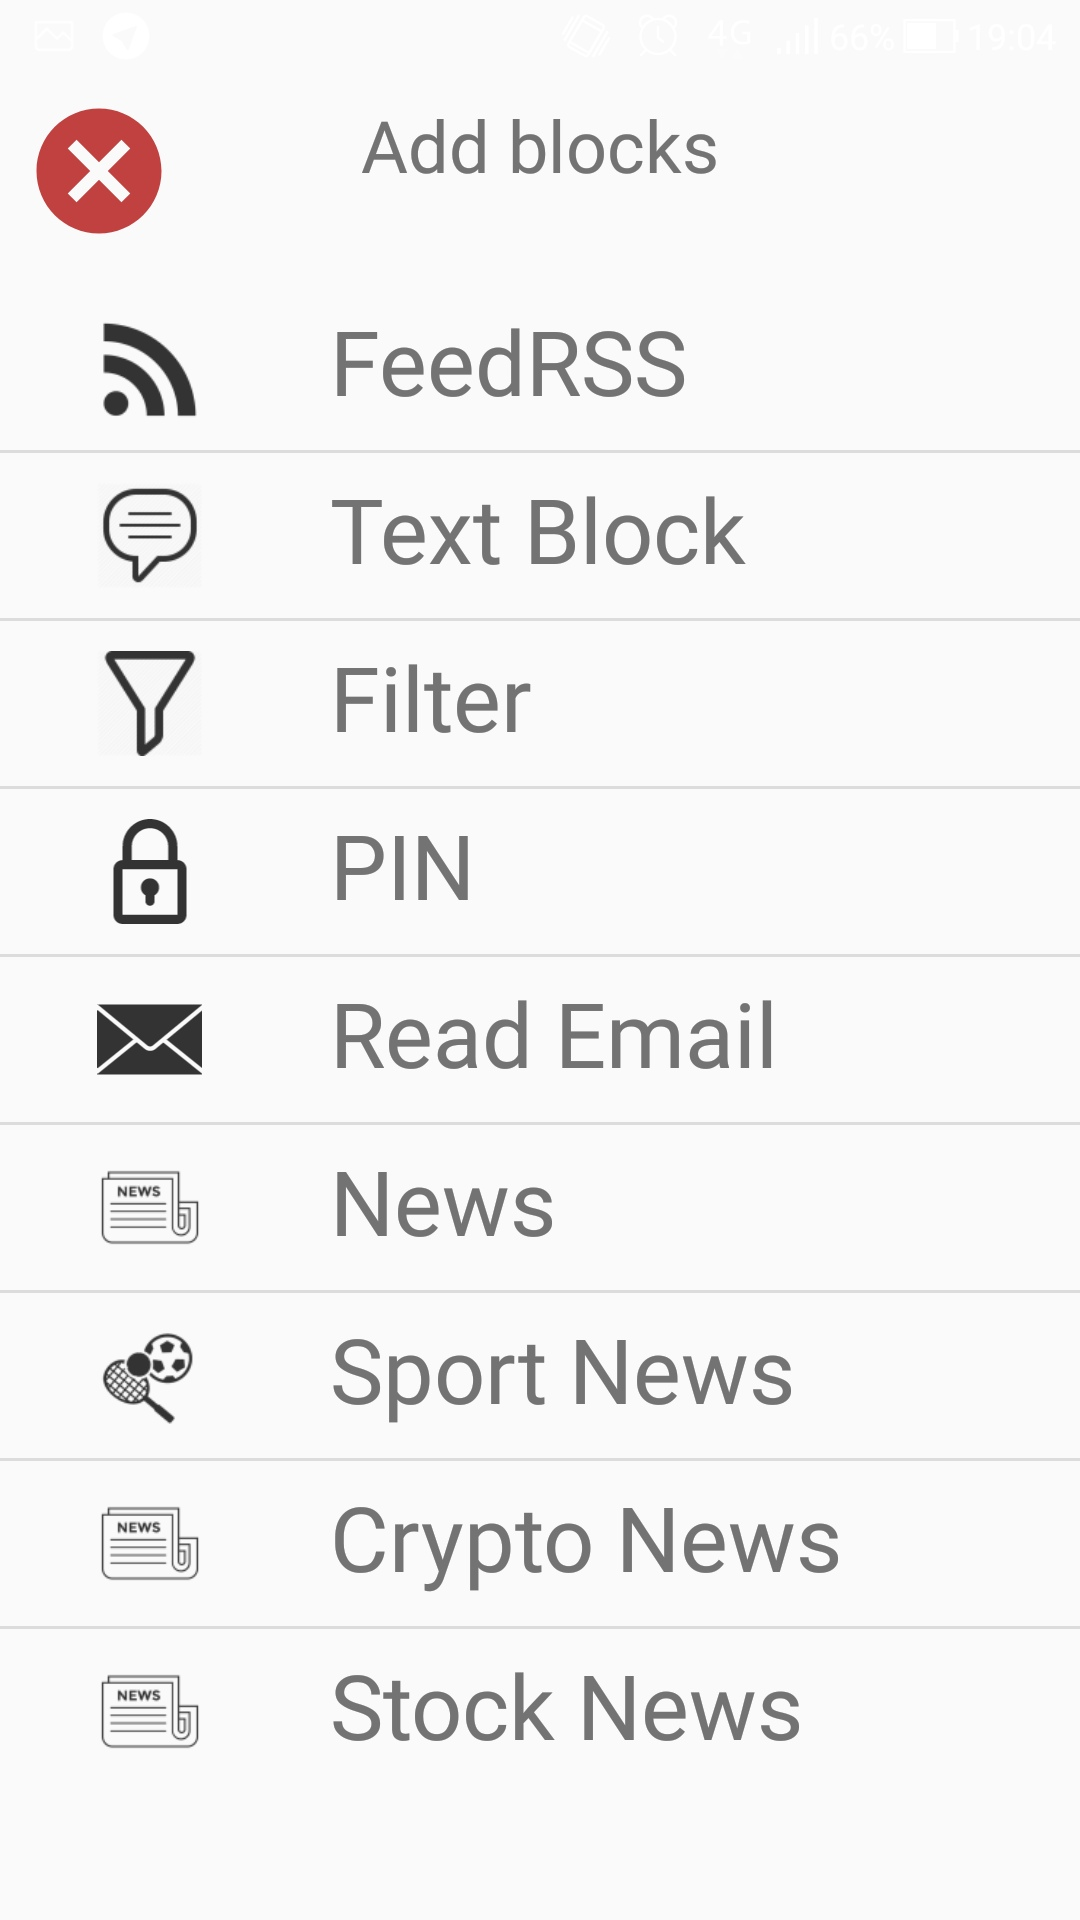
\includegraphics[scale=0.2]{images/ListBlocks.jpg}
	\caption{}
\end{figure}

\subsubsection{Blocco Amazon Music}
Questo blocco consente all'utente di ascoltare un brano, un'album o una playlist da Amazon Music tramite il proprio dispositivo Alexa.

\subsubsection{Blocco Borsa}

\subsubsection{Blocco Calendar}
Il blocco calendario permette all'utente di ascoltare o aggiungere i suoi appuntamenti di Google calendar tramite l'Amazon echo.

\subsubsection{Blocco Crypto}

\subsubsection{Blocco FeedRSS}
Questo blocco permette all'utente di inserire un qualsiasi feedRSS e successivamente far riprodurre al dispositivo Alexa il suo contenuto.
\begin{enumerate}
	\item Inserire nell'apposito campo di testo l'URL del feedRSS
	\item Confermare e salvare cliccando sul pulsante ADD
\begin{figure}[!ht]
	\centering
	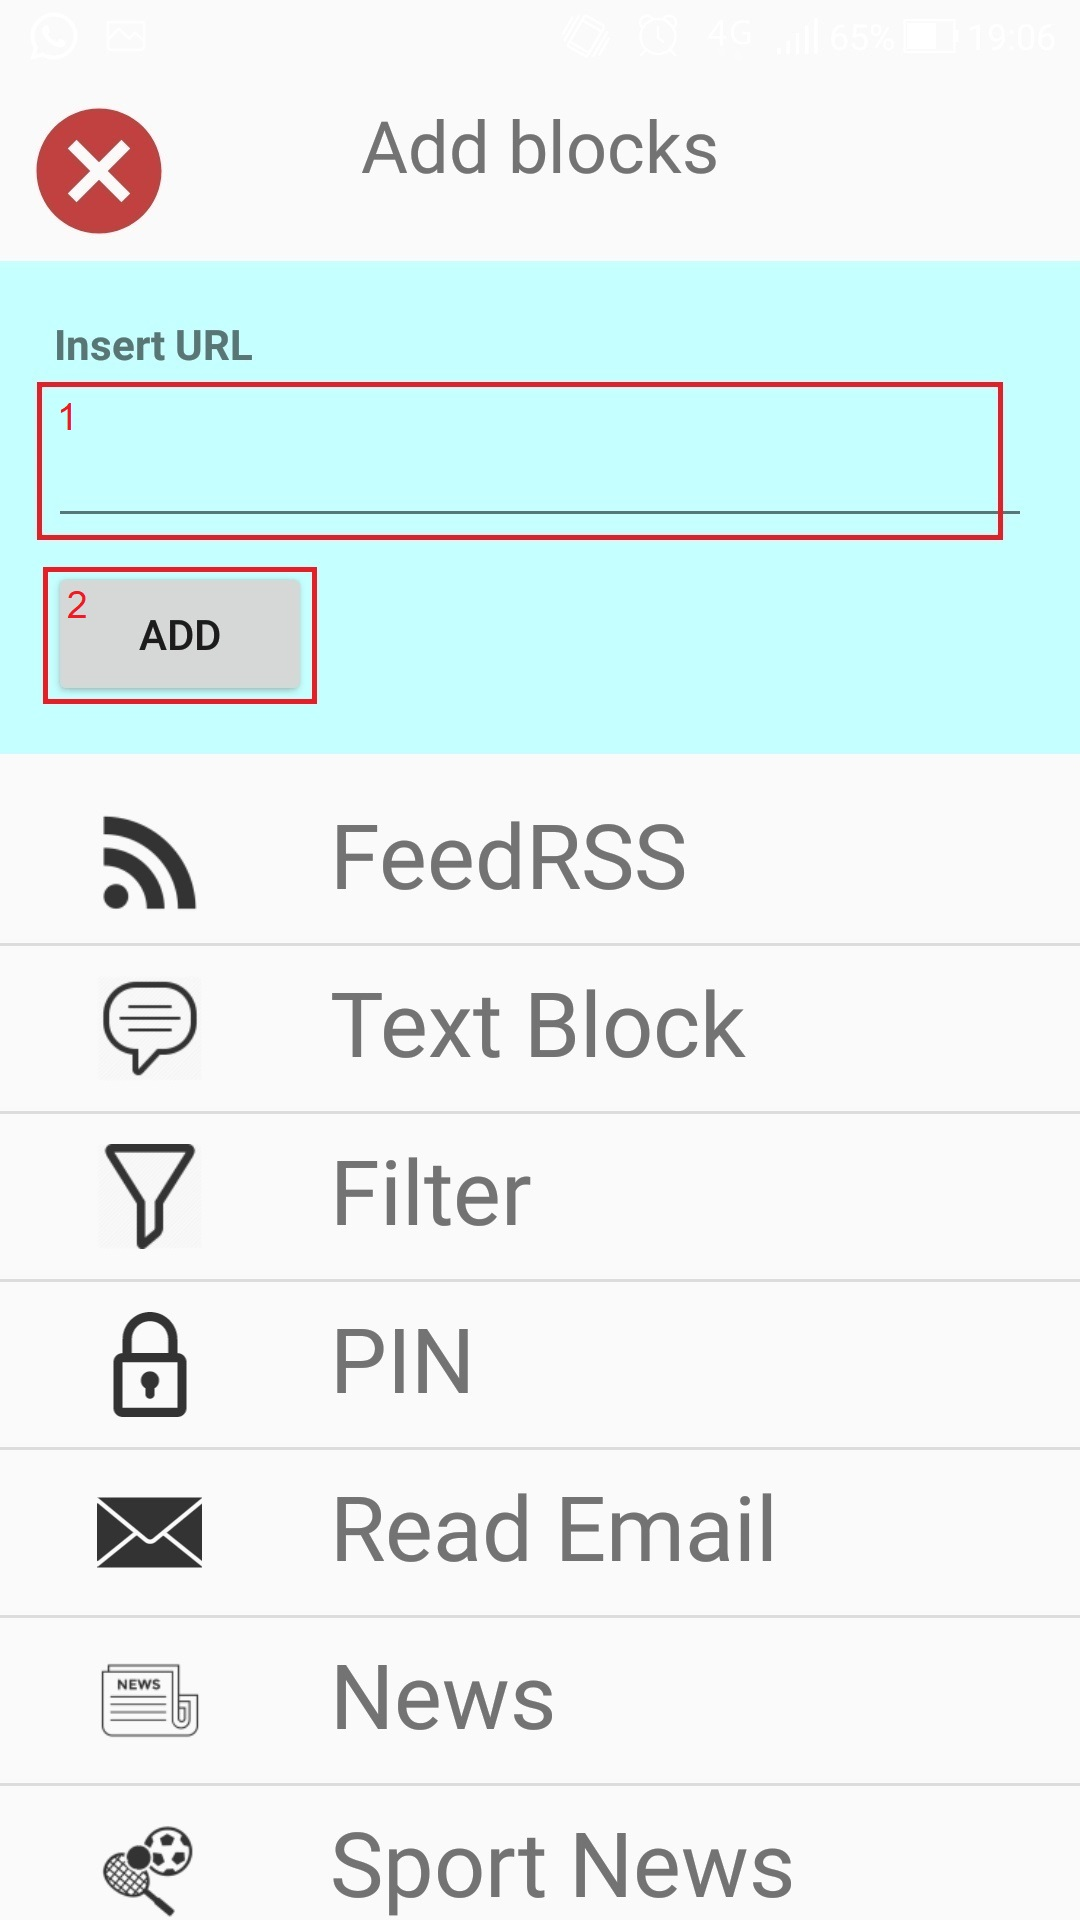
\includegraphics[scale=0.2]{images/BlockFeedRSS.jpg}
	\caption{Blocco FeedRSS}
\end{figure}
\end{enumerate}

\subsubsection{Blocco Filter}
Consente di impostare il numero limite di elementi che un determinato blocco deve considerare. \\
\textbf{NOTA BENE:} il blocco filtro è applicabile solo ai seguenti blocchi: Borsa, Crypto, FeedRSS, News, Readmail e Sport.

\subsubsection{Blocco List}
Questo blocco permette all'utente di creare, aggiungere e modificare degli elementi di testo ad una lista.
È possibile modificare la lista tramite app oppure tramite interazione con l'Amazon Echo.

\subsubsection{Blocco News}
Tale blocco consente all'utente di ascoltare le ultime news prese da un sito a scelta tra i seguenti: Sky, Google News, Ansa, BBC, CNBC e Wall Street.

\begin{figure}[!ht]
	\centering
	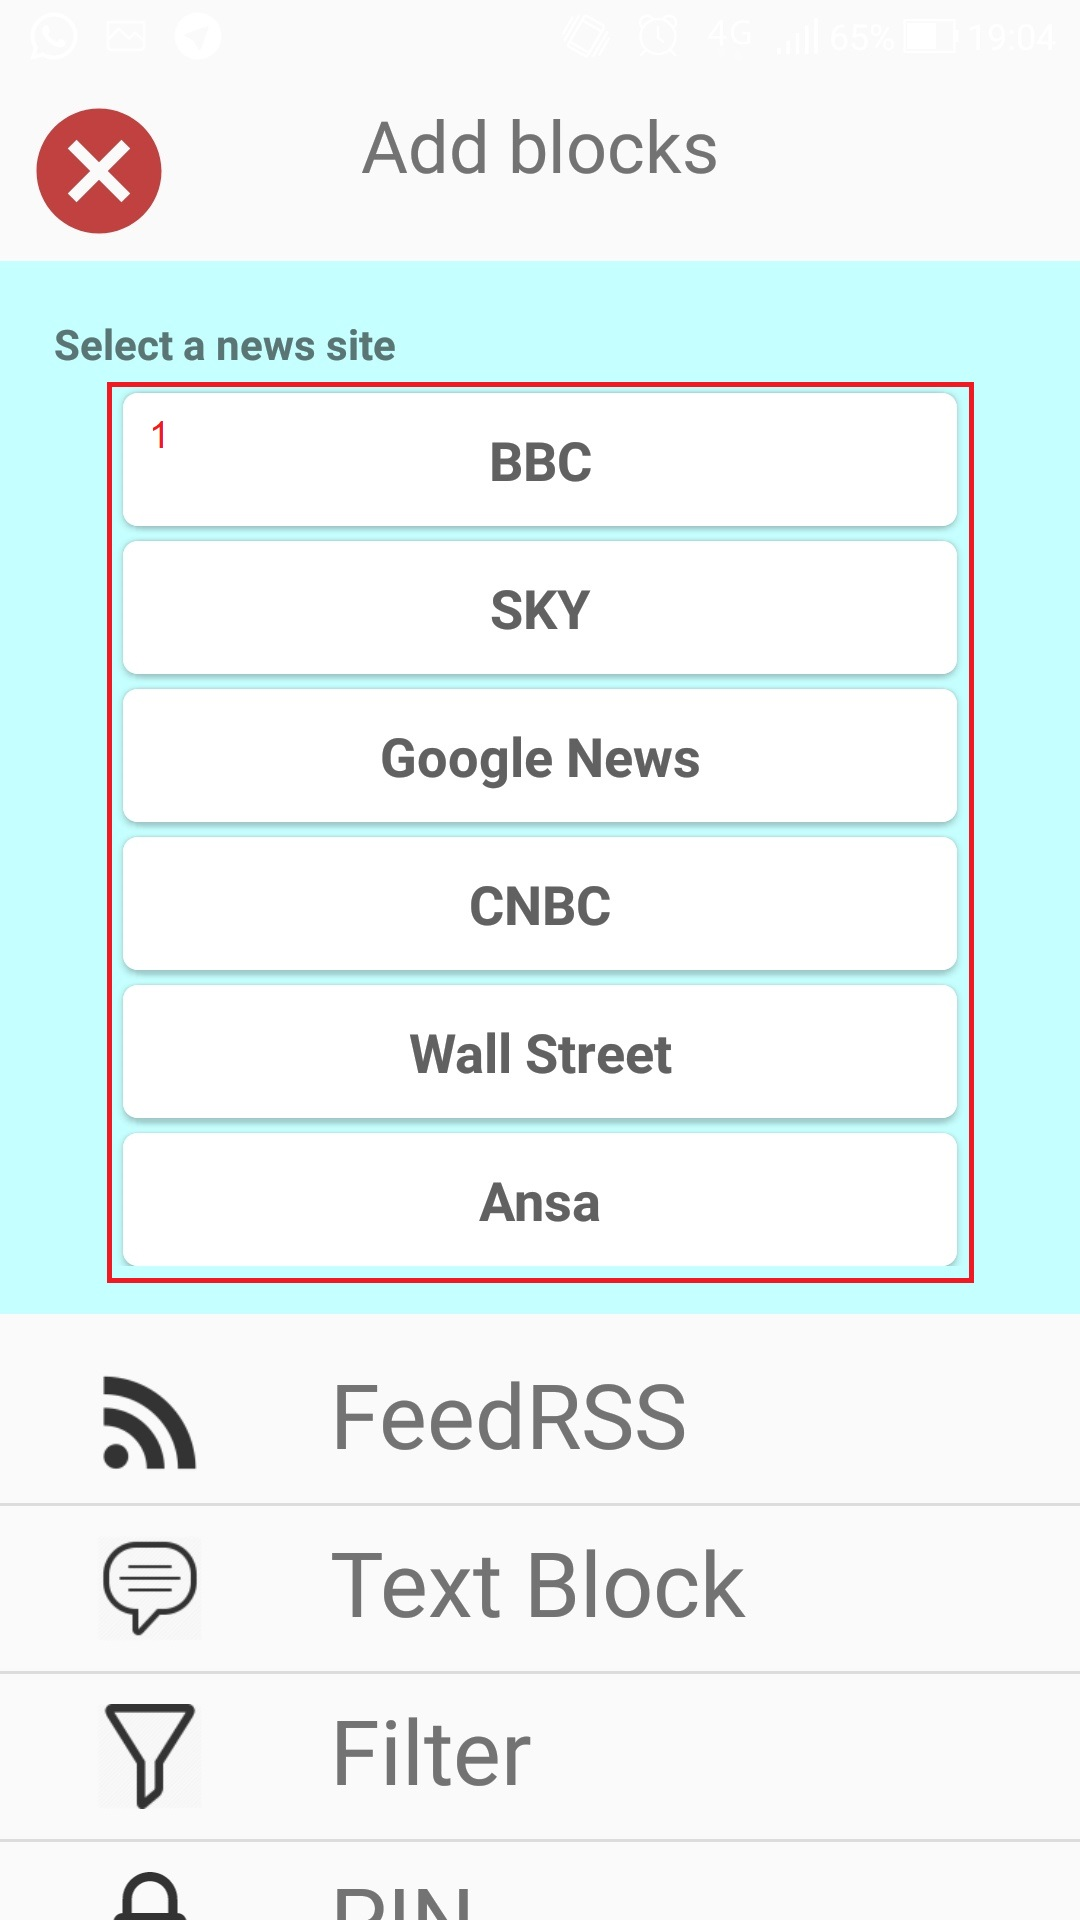
\includegraphics[scale=0.2]{images/BlockNews.jpg}
	\caption{Blocco News}
\end{figure}

\subsubsection{Blocco PIN}
Lo scopo di questo blocco è quello di effettuare una sorta di autenticazione dell'utente per l'esecuzione di alcuni blocchi, ovvero: calendar, ReadMail, SendEmail e Twitter in modo da avere un minimo di privacy per l'utente.

\begin{figure}[!ht]
	\centering
	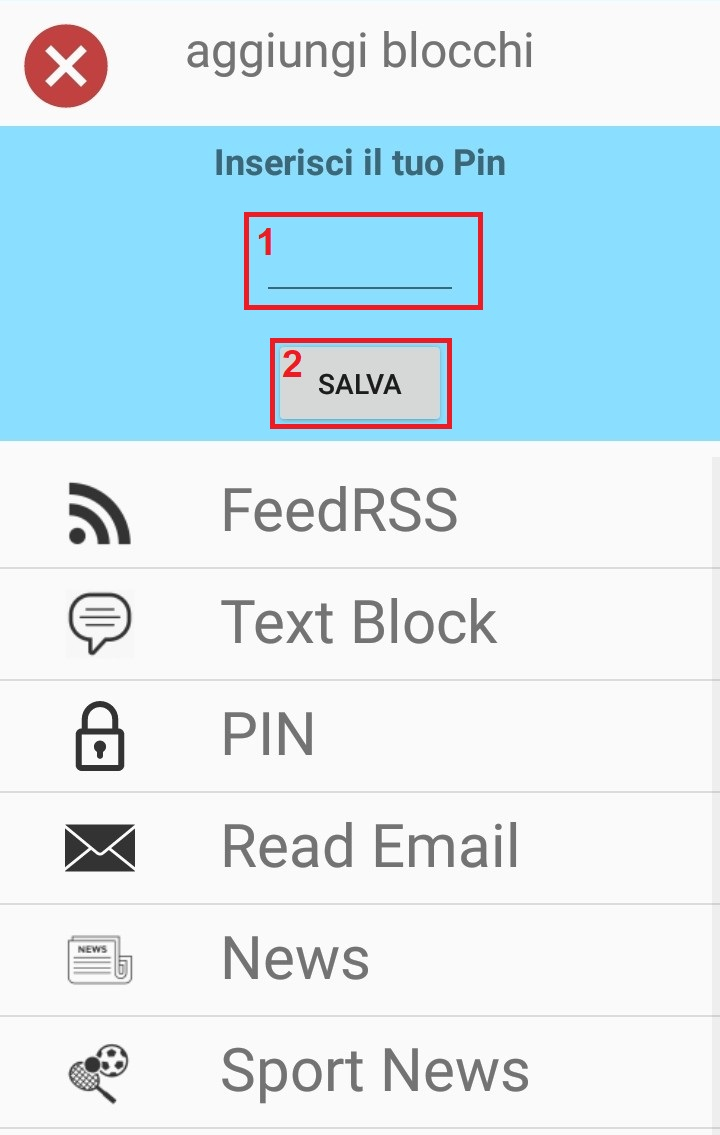
\includegraphics[scale=0.4]{images/BlockPIN.jpg}
	\caption{Blocco PIN}
\end{figure}

\subsubsection{Blocco ReadEmail}
Con questo blocco l'utente può ascoltare tramite Alexa le sue email, di Gmail, non ancora lette.


\subsubsection{Blocco SendEmail}

\subsubsection{Blocco Sport}
Con l'aggiunta di questo blocco l'utente potrà ascoltarsi le ultime news riguardanti uno sport sua scelta tra i seguenti: tennis, calcio, basket americano, formula1, football americano e motogp.

\begin{figure}[!ht]
	\centering
	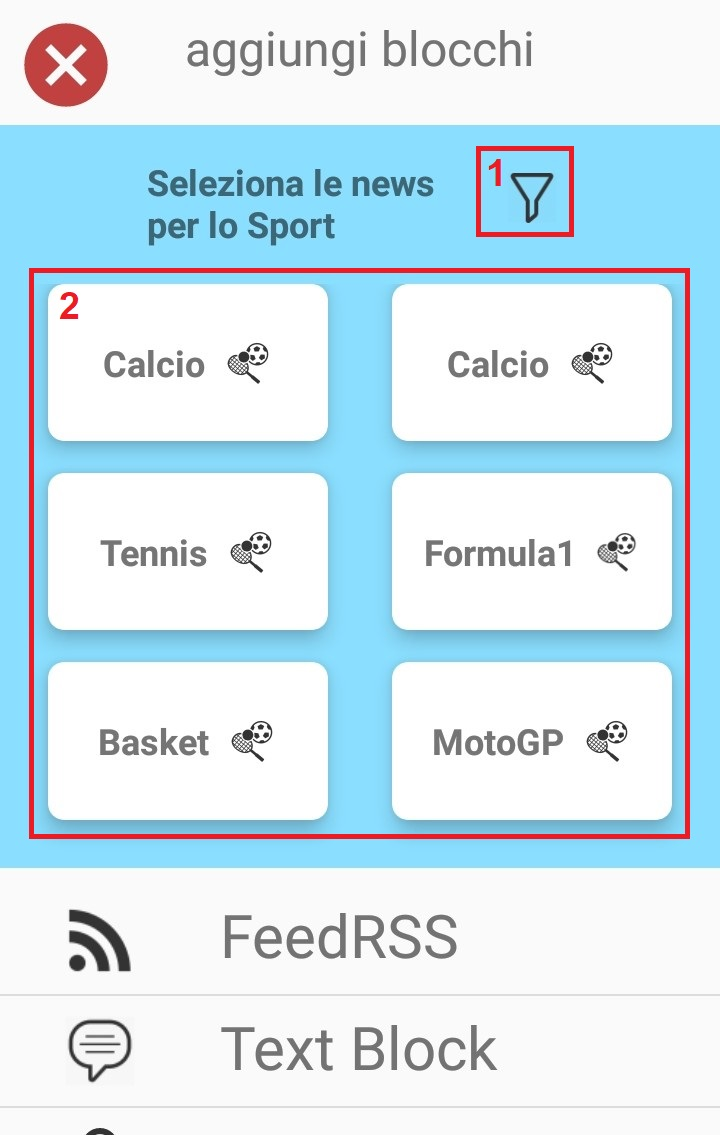
\includegraphics[scale=0.2]{images/BlockSport.jpg}
	\caption{Blocco sport}
\end{figure}

\subsubsection{Blocco Telegram}
Il blocco Telegram consente all'utente iscritto al servizio di messaggistica Telegram di inviare messaggi e file audio ad un'altra persona o gruppo di persone.

\subsubsection{Blocco TextBox}
Tale blocco consente all'utente di inserire nel proprio workflow un blocco contenente del testo.

\begin{figure}[!ht]
\centering
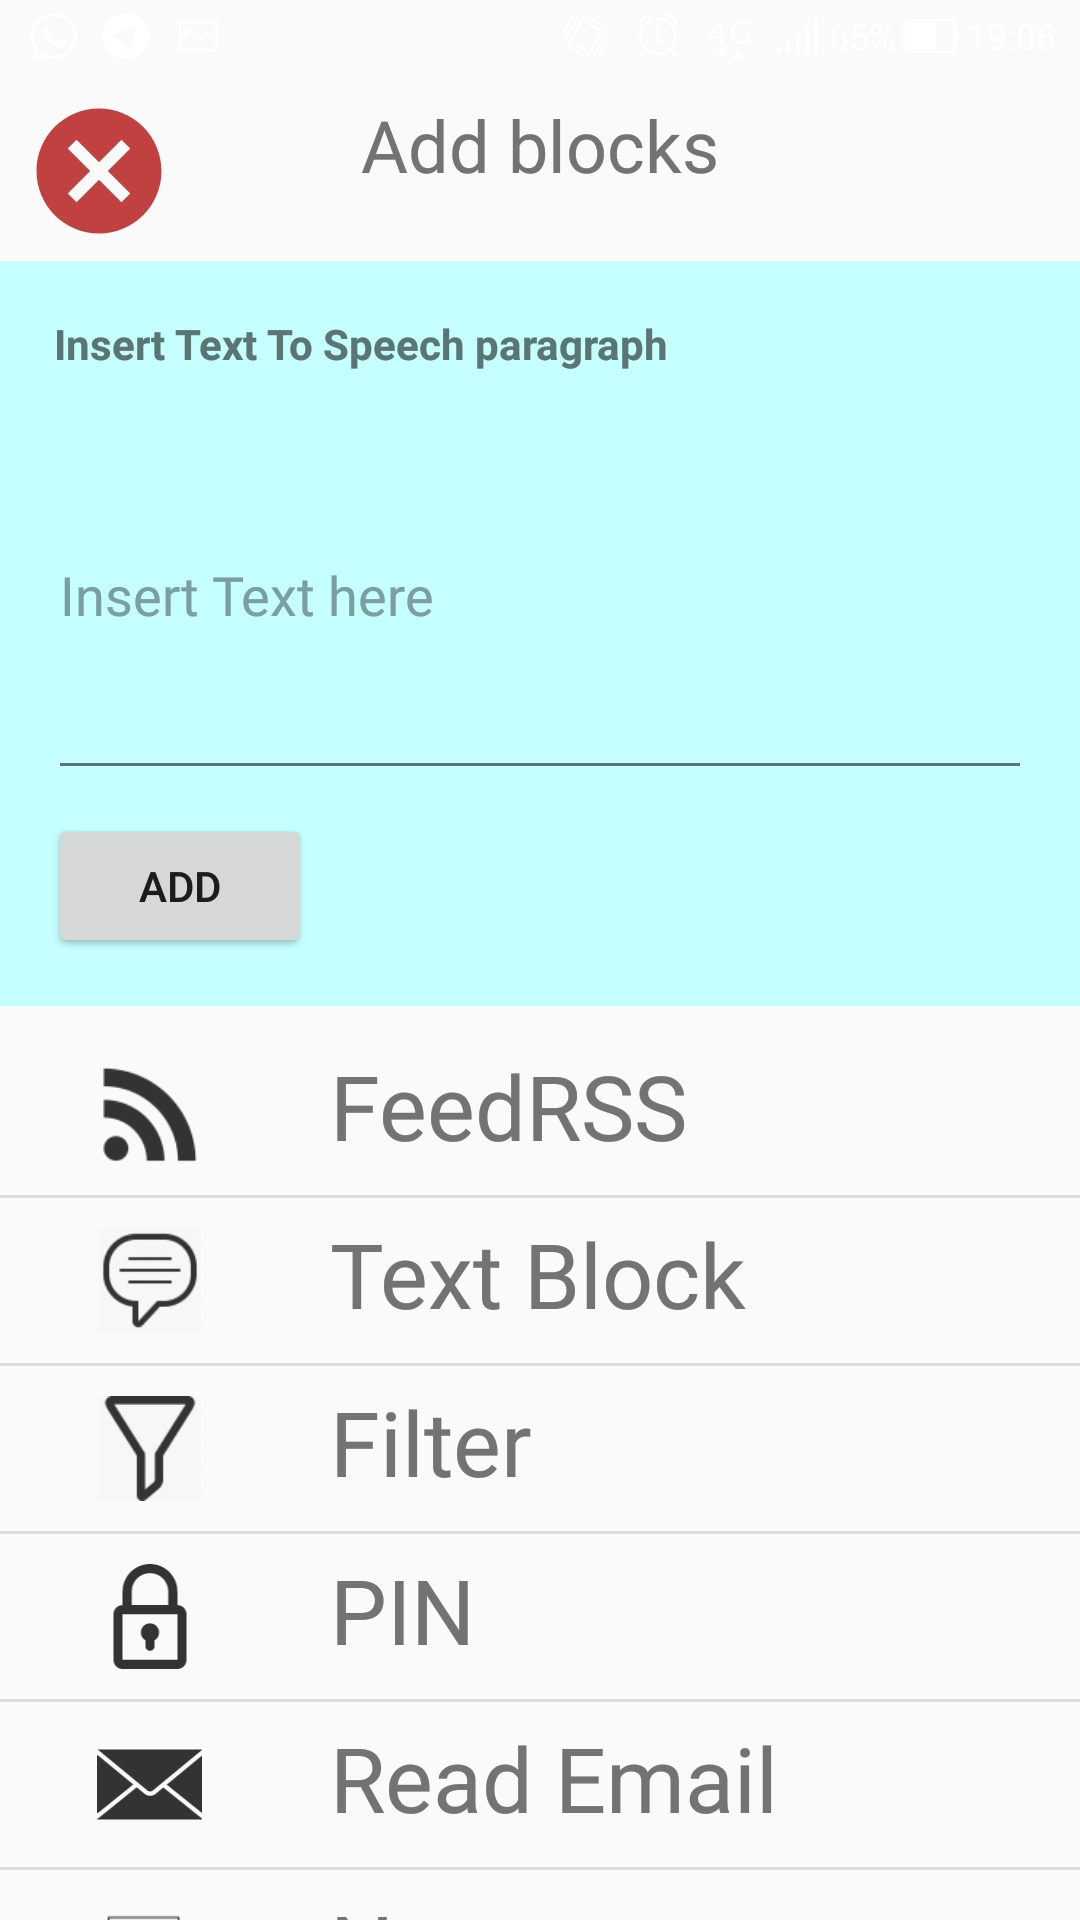
\includegraphics[scale=0.2]{images/BlockTextToSpeech}
\caption{}
\end{figure}

\subsubsection{Blocco Twitter}


\subsubsection{Blocco Weather}
Il blocco Weather consente all'utente di sapere che meteo c'è in una determinata città.
